\documentclass[11pt]{article}
\usepackage[letterpaper,margin=.8in]{geometry}
\usepackage[T1]{fontenc}
\usepackage{lmodern,microtype,amsmath,amssymb,graphicx,booktabs}
\usepackage[hidelinks]{hyperref}
\setlength{\parindent}{1em}
\setlength{\parskip}{3pt}
\setlength{\abovedisplayskip}{7pt plus 2pt minus 2pt}
\setlength{\belowdisplayskip}{7pt plus 2pt minus 2pt}
\newcommand{\notesubsection}[1]{\par\addvspace{6pt}\noindent\textbf{#1.}\nobreakspace}
\newcommand{\R}{\mathbb R}
\newcommand{\asinh}{\operatorname{arsinh}}
\hypersetup{pdftitle={How finely can we measure a curve?},pdfauthor={Jonathan R. Landers}}
\begin{document}
\begin{center}
{\LARGE How finely can we measure a curve?\par}
\smallskip
{\large A parabola, a minimum distance, and a finite error\par}
\medskip
Jonathan R. Landers\quad---\quad November 25, 2026
\end{center}

\section{Arc length with a minimum distance}
\notesubsection{A curve and its chords}
A parabola makes a useful place to begin. Its equation is simple,
its length is not just the distance between its endpoints, and its bend
can be followed with a pencil. Start with $y=x^2$: the vertex is $(0,0)$,
the curve opens upward, and reflection across the $y$-axis leaves it
unchanged. How long is a chosen piece of it? And if distinct positions
cannot be arbitrarily close, how accurately can little right triangles
answer that question?

We use dimensionless coordinates in a fixed length unit $\ell$:
$x=X/\ell$, $y=Y/\ell$. Thus the physical parabola is $Y=X^2/\ell$.
Lengths and errors below acquire physical units on multiplication by
$\ell$; a physical minimum distance $k_{\rm phys}$ is written
$k=k_{\rm phys}/\ell$. This convention keeps expressions such as
$\sqrt{k}$ unambiguous.

For a continuously differentiable graph $y=f(x)$ on $[a,b]$, its
Euclidean arc length is
\begin{equation}\label{eq:length}
 L=\int_a^b\sqrt{1+f'(x)^2}\,dx.
\end{equation}
For the parabola, $f'(x)=2x$, and an antiderivative is
\begin{equation}\label{eq:primitive}
 F(x)=\frac{x}{2}\sqrt{1+4x^2}+\frac14\asinh(2x),
 \qquad L=F(b)-F(a).
\end{equation}
Here $\asinh z=\log(z+\sqrt{1+z^2})$. On $[-3,3]$ this gives
\begin{equation}\label{eq:exact}
 L=3\sqrt{37}+\tfrac12\log(6+\sqrt{37})
   =19.494177517\ldots\,.
\end{equation}

The integral has a concrete geometric origin. Choose
$a=x_0<x_1<\cdots<x_N=b$, and join successive points
$P_i=(x_i,f(x_i))$. The segment $P_{i-1}P_i$ is the hypotenuse of
a right triangle with horizontal leg $\Delta x_i=x_i-x_{i-1}$ and
vertical leg $|\Delta y_i|=|f(x_i)-f(x_{i-1})|$, using the corner
$(x_i,f(x_{i-1}))$. The total chord length is
\begin{equation}\label{eq:polygon}
 L_N=\sum_{i=1}^N\sqrt{(\Delta x_i)^2+(\Delta y_i)^2}.
\end{equation}
Every chord is no longer than its intervening arc. Refining a partition
cannot decrease $L_N$, and as its largest width tends to zero,
$L_N\to L$. For $f(x)=x^2$, the factorization
$\Delta y_i=(x_i+x_{i-1})\Delta x_i$ makes each summand
$\Delta x_i\sqrt{1+(x_i+x_{i-1})^2}$.

\begin{figure}[htbp]
\centering
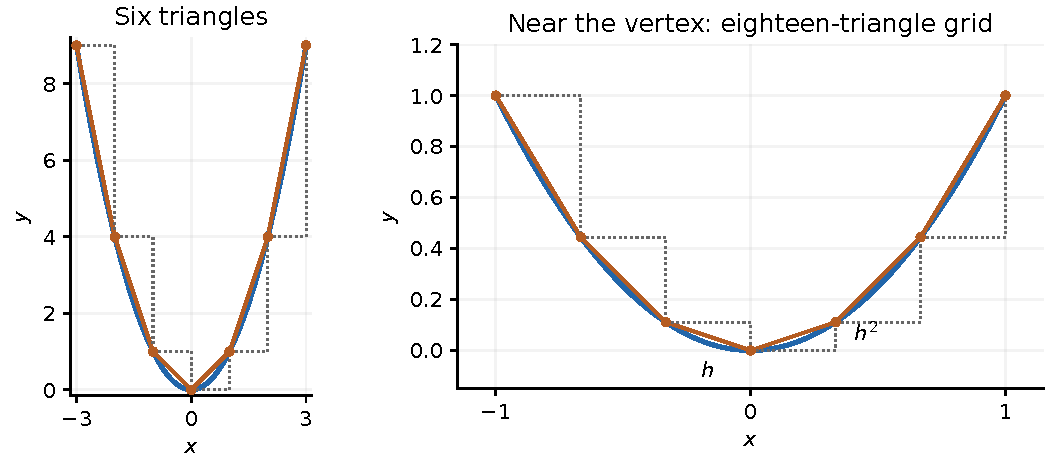
\includegraphics[width=.97\linewidth]{figures/parabola_triangles.pdf}
\par\smallskip
\begin{minipage}{.95\linewidth}\small
\textbf{Figure 1.} The smooth parabola and its chords; dotted legs complete
the right triangles. Left: six chords over $[-3,3]$. Right: the central
part of an eighteen-chord partition, where the smallest vertical leg is
$h^2$. The panels have equal horizontal and vertical coordinate scales.
\end{minipage}
\end{figure}

\notesubsection{When refinement has to stop}
Now impose the hypothesis used in the minimum-distance papers
\cite{landers,triangles}: distinct physical positions have Euclidean
separation at least $k>0$. The smooth graph remains a reference curve;
its entire continuum of points is not being declared physical. Suppose
the three vertices of every approximating right triangle are required
positions. Its two legs must then satisfy
\begin{equation}\label{eq:legs}
 \Delta x_i\ge k,\qquad |\Delta y_i|\ge k,
 \qquad c_i=\sqrt{(\Delta x_i)^2+(\Delta y_i)^2}\ge\sqrt2\,k.
\end{equation}
Requiring only $c_i\ge k$ would miss the obstruction: a long chord can
still have an impermissibly short leg. A horizontal chord has a zero
vertical leg and does not provide a nondegenerate right triangle.

Adding the horizontal legs and the hypotenuses gives, respectively,
$Nk\le b-a$ and $N\sqrt2\,k\le L_N\le L$. Consequently every
admissible partition obeys the general count bound
\begin{equation}\label{eq:general-count}
 \boxed{N\le\left\lfloor\min\left\{
 \frac{b-a}{k},\frac{L}{\sqrt2\,k}\right\}\right\rfloor.}
\end{equation}
This is an upper bound, not an existence theorem. Leg constraints need
not be simultaneously achievable, and a prescribed discrete position
space might not contain the proposed vertices at all. Nor is a continuum
limit available by increasing $N$ at fixed $k$ on a fixed interval.

To obtain an exact count for a specified construction, keep the horizontal
steps equal. Put $h_n=(b-a)/n$. The largest uniform count passing the
individual-triangle constraints is
\begin{equation}\label{eq:uniform-generic}
 N_{\rm unif}=\max\left(\{0\}\cup\left\{n\in\mathbb N:
 h_n\ge k,\ \min_{1\le i\le n}
 |f(a+ih_n)-f(a+(i-1)h_n)|\ge k\right\}\right).
\end{equation}
The value zero records that no such partition exists. With the specified
corner choice, the leg inequalities also ensure separation of the whole
vertex set: different horizontal coordinates differ by at least $k$;
at a shared coordinate the only possible distinct vertices are the curve
point and its corner, separated by a vertical leg. Coincident vertices
are identified. Membership in a preassigned position space is still an
additional requirement.

For $f(x)=x^2$, the vertical increment has magnitude
\begin{equation}\label{eq:parabola-increment}
 |\Delta y_i|=h_n\,|2a+(2i-1)h_n|.
\end{equation}
On our symmetric interval $[-3,3]$, every odd $n$ has a central chord
joining points of equal height and fails the vertical-leg condition.
For even $n$, the two smallest vertical legs, next to the vertex, have
length $h_n^2$. All other vertical legs are larger. Hence the conditions
are exactly
\begin{equation}\label{eq:even}
 n\ \text{even},\qquad h_n=6/n\ge k,\qquad h_n^2\ge k.
\end{equation}
The maximum uniform count is therefore
\begin{equation}\label{eq:nk}
 \boxed{N(k)=2\left\lfloor\min\left\{
 \frac3k,\frac3{\sqrt{k}}\right\}\right\rfloor.}
\end{equation}
For $0<k\le3$ this is at least two; for $k>3$ no uniform partition
of this kind exists. At $k=1$ it permits six triangles, and at $k=0.1$
it permits eighteen. Writing $n=2m$, every triangle vertex lies in
$h_n\mathbb Z\times h_n^2\mathbb Z$; conditions \eqref{eq:even}
therefore give a second direct check that all distinct vertices are
mutually separated by at least $k$. This constructs a finite admissible
position set, without assuming a physical lattice. It does not optimize
over nonuniform placements.

\notesubsection{The price of stopping}
How much length is lost when refinement stops? Define
\begin{equation}\label{eq:error}
 E_N=L-L_N\ge0.
\end{equation}
For a $C^2$ graph with $|f''|\le M$, every partition satisfies
\begin{equation}\label{eq:bound}
 0\le E_N\le\frac{M^2}{24}\sum_{i=1}^N(\Delta x_i)^3
 \le\frac{M^2(b-a)\delta^2}{24},\qquad
 \delta=\max_i\Delta x_i.
\end{equation}
To prove this, on a cell of width $h$ put $p=f'$, $\bar p=h^{-1}\int p$,
and $G(p)=\sqrt{1+p^2}$. Its chord length is $hG(\bar p)$.
Since $0<G''\le1$ and $|p(x)-p(t)|\le M|x-t|$, its arc excess satisfies
\[
 \int G(p)\,dx-hG(\bar p)
 \le\tfrac12\int(p-\bar p)^2dx
 =\frac1{4h}\iint(p(x)-p(t))^2dx\,dt
 \le\frac{M^2h^3}{24}.
\]
Summing proves \eqref{eq:bound}. For uniform $h=(b-a)/N$, the bound
is $M^2(b-a)^3/(24N^2)$, and midpoint expansion gives
\begin{equation}\label{eq:generic-asymptotic}
 E_N=\frac{h^2}{24}\int_a^b
 \frac{f''(x)^2}{(1+f'(x)^2)^{3/2}}\,dx+o(h^2),
 \qquad h\to0.
\end{equation}
For the parabola, take $N=N(k)\ge2$ and $h=6/N$. Its chord sum is
exactly the midpoint rule for $g(x)=\sqrt{1+4x^2}$, giving
\begin{equation}\label{eq:exact-error}
 \boxed{E(k)=3\sqrt{37}+\tfrac12\log(6+\sqrt{37})
 -h\sum_{i=1}^{N(k)}\sqrt{1+[-6+(2i-1)h]^2}.}
\end{equation}
Since $M=2$, \eqref{eq:bound} gives $E(k)\le h^2$. More precisely,
$g'(3)-g'(-3)=24/\sqrt{37}$, and the midpoint expansion gives
\begin{equation}\label{eq:asymptotic}
 E(k)=\frac{h^2}{24}\bigl(g'(3)-g'(-3)\bigr)+O(h^4)
     =\frac{h^2}{\sqrt{37}}+O(h^4).
\end{equation}
\begin{center}
\small
\begin{tabular}{rrrr}
\toprule
Cutoff $k$ & Triangles $N(k)$ & Chord estimate $L_N$ & Error $E(k)$\\
\midrule
1 & 6 & 19.351021472 & 0.143156045 \\
0.1 & 18 & 19.475917708 & 0.018259809 \\
0.01 & 60 & 19.492533523 & 0.001643994 \\
\bottomrule
\end{tabular}

\end{center}
The table uses the exact sum. As $k\downarrow0$, \eqref{eq:nk} implies
$h^2\sim k$, including the floor's effect. Therefore
\begin{equation}\label{eq:k-error}
 \boxed{E(k)\sim k/\sqrt{37}=0.164398987\ldots\,k.}
\end{equation}
The flat vertex explains the scaling: its shortest vertical leg forces
$h\ge\sqrt{k}$. This is the stated construction's error, not a universal
lower bound for all estimators. The analytic integral remains available;
the distance gap removes this construction's unlimited refinement.

\section{Main Result}
Stopping refinement need not mean discarding the triangles' remaining
information. Two neighboring hypotenuses also tell us how the average
slope changes across their shared vertex. If that change nearly exhausts
an independently known bound on slope variation, little freedom remains
for the smooth arc between the samples. We can turn this observation into
an explicit error certificate at the existing sampling scale.

\notesubsection{Angles and reconstruction}
Let $f\in C^2([u-h,u+h])$, $h>0$, and suppose $|f''|\le M$ for a
known $M>0$. Write $I_1=[u-h,u]$, $I_2=[u,u+h]$ and
$c_1=u-h/2$, $c_2=u+h/2$. The measured slopes are
\begin{equation}
 m_1=\frac{f(u)-f(u-h)}h=\tan\theta_1,\qquad
 m_2=\frac{f(u+h)-f(u)}h=\tan\theta_2,
\end{equation}
where the signed angles lie in $(-\pi/2,\pi/2)$. Set $s=1$ when
$m_2\ge m_1$ and $s=-1$ otherwise, and define
\begin{equation}\label{eq:deficit}
 D=Mh-|m_2-m_1|,\qquad q_i(x)=m_i+sM(x-c_i),\qquad
 \widehat L=\sum_{i=1}^2\int_{I_i}\sqrt{1+q_i(x)^2}\,dx.
\end{equation}
Each $q_i$ has the measured mean slope and changes at the largest
permitted rate in the observed direction. Integrating it reconstructs
a quadratic arc through that cell's endpoints. These arcs meet in
position, with derivative jump of magnitude $D$ at their shared vertex.

\noindent\textit{For every graph satisfying these assumptions,}
\begin{equation}\label{eq:main}
 \boxed{0\le D\le Mh,\qquad
 |L_{12}-\widehat L|\le2hD
 =2h\bigl(Mh-|\tan\theta_2-\tan\theta_1|\bigr),}
\end{equation}
\textit{where $L_{12}$ is its length on the two cells. If $D=0$, then
$f''=sM$ throughout, the three sampled values determine the graph
uniquely, and $L_{12}=\widehat L$.}

The estimator requires only elementary functions. With
$H(z)=\tfrac12[z\sqrt{1+z^2}+\asinh z]$, substitution gives
\begin{equation}\label{eq:evaluation}
 \widehat L=\frac1M\sum_{i=1}^2
 \bigl[H(m_i+Mh/2)-H(m_i-Mh/2)\bigr].
\end{equation}
This holds for either sign $s$. If $M=0$, the graph is affine and its
chord length is exact.

The reconstruction gives a concrete interpretation of the correction.
A chord replaces all slopes in its cell by their mean. The functions
$q_i$ restore slope variation while preserving the same endpoints.
Because $G(z)=\sqrt{1+z^2}$ is convex, each reconstructed arc is at
least as long as its chord. The uncertainty is how closely this
reconstructed variation follows the actual curve. Equation
\eqref{eq:main} controls that uncertainty using the observed turn.

The angles enter through their slopes $\tan\theta_i$, since the
sampling intervals have equal horizontal width. In a smooth graph the
slope changes continuously, whereas the chords record successive cell
averages. Their difference measures the integrated change that must
occur between those cells. When it reaches the permitted maximum,
equality leaves precisely the quadratic reconstruction.

\notesubsection{Proof}
To prove this, write $p=f'$. By the fundamental theorem of calculus,
each chord slope is the average of $p$ over its cell. Moving the
averaging interval one step to the right gives
\[
 m_2-m_1=\frac1h\int_{u-h}^{u}[p(x+h)-p(x)]\,dx,
 \qquad |p(x+h)-p(x)|\le Mh.
\]
Thus $|m_2-m_1|\le Mh$, establishing the stated range of $D$.
To measure departure from the reconstructed slope, remove its maximal
linear trend by putting
$r(x)=sp(x)-M(x-u)$. Since $r'=sf''-M\le0$, $r$ is nonincreasing.
Its cell averages satisfy
\[
 \bar r_1=sm_1+Mh/2,\qquad \bar r_2=sm_2-Mh/2,
 \qquad \bar r_1-\bar r_2=D.
\]
With $r_0=r(u)$, monotonicity gives $r\ge r_0$ on $I_1$ and
$r\le r_0$ on $I_2$, so
\[
 \sum_i\int_{I_i}|r-r_0|\,dx
 =h(\bar r_1-r_0)+h(r_0-\bar r_2)=hD,
 \qquad \sum_i h|\bar r_i-r_0|=hD.
\]
These identities use the shared vertex to control both cells together.
The first measures departure from $r_0$ inside the cells, and the second
measures how far their averages lie from that same value. Since
$s(p-q_i)=r-\bar r_i$, the triangle inequality gives
\[
 \sum_i\int_{I_i}|p-q_i|\,dx
 \le\sum_i\int_{I_i}|r-r_0|\,dx
       +\sum_i h|\bar r_i-r_0|.
\]
Consequently,
\begin{equation}\label{eq:slope-error}
 \sum_i\int_{I_i}|p-q_i|\,dx
 =\sum_i\int_{I_i}|r-\bar r_i|\,dx\le2hD.
\end{equation}
Finally $G(z)=\sqrt{1+z^2}$ satisfies
$|G'(z)|=|z|/\sqrt{1+z^2}\le1$. Therefore
\[
 |L_{12}-\widehat L|
 \le\sum_i\int_{I_i}|G(p)-G(q_i)|\,dx
 \le\sum_i\int_{I_i}|p-q_i|\,dx\le2hD.
\]
This proves the length bound. When $D=0$, the continuous nonnegative
integrands in \eqref{eq:slope-error} have zero integral, so $p=q_i$
on both cells. Thus $f''=sM$ throughout. Integrating twice gives
$f(x)=sMx^2/2+ax+b$, and the sampled values determine the remaining
affine coefficients. This proves the equality and uniqueness claims.

\notesubsection{A certified improvement}
The quantity $D$ measures the freedom left after the observed turn.
A slope change close to $Mh$ leaves little room to depart from the
maximal linear trend. Combining this information with the earlier
chord bound makes the improvement explicit. For
$C=h\sqrt{1+m_1^2}+h\sqrt{1+m_2^2}$, equations
\eqref{eq:bound} and \eqref{eq:main} imply
\begin{equation}\label{eq:intersection}
 \boxed{\max\{C,\widehat L-2hD\}\le L_{12}\le
 \min\{C+M^2h^3/12,\widehat L+2hD\}.}
\end{equation}
Its midpoint has absolute error at most half the interval width.
The width is at most the earlier $M^2h^3/12$, and the angular interval
alone has width $4hD$. Thus $D<M^2h^2/48$ suffices for a strict
reduction. The combined interval can also improve the bound when this
sufficient condition fails, as Figure 2 illustrates.

For a longer chain, group equal-width cells into disjoint adjacent pairs.
Writing $[A_j,B_j]$ for each pair's interval in \eqref{eq:intersection},
additivity gives
\[
 \left|L-\sum_j\widehat L_j\right|\le2h\sum_jD_j,
 \qquad \sum_jA_j\le L\le\sum_jB_j.
\]
An unpaired cell retains its chord bound. Using disjoint pairs ensures
that each arc is counted once. The midpoint of the summed interval has
absolute error at most half its width.

\notesubsection{The parabola and a quartic comparison}
For the parabola, even the three vertices $(-3,9),(0,0),(3,9)$ suffice
when $M=2$ is supplied independently. Here $h=3$, $m_1=-3$, $m_2=3$,
and $D=0$. The result forces $f''=2$ and then $f=x^2$, recovering
$L=19.494177517\ldots$ exactly from a chord sum of
$6\sqrt{10}=18.973665961\ldots$. At $k=3$ these are the two
triangles allowed by \eqref{eq:nk}, with legs $3$ and $9$.
The angular calculation recovers the missing $0.520511556\ldots$
without inserting another physical vertex.

To see the certificate away from equality, keep the three horizontal
sample coordinates and take $f_\varepsilon=x^2-\varepsilon x^4$ on
$[-3,3]$, with $0\le\varepsilon\le1/27$. Then
$f_\varepsilon''=2-12\varepsilon x^2\in[-2,2]$, so $M=2$ remains
valid. The slopes are $m_2=-m_1=3-27\varepsilon$, giving
$D=54\varepsilon$ and error radius $2hD=324\varepsilon$.
The vertical legs are at least $6$, retaining admissibility at $k=3$.

\par\medskip\noindent\begin{minipage}{\linewidth}
\centering
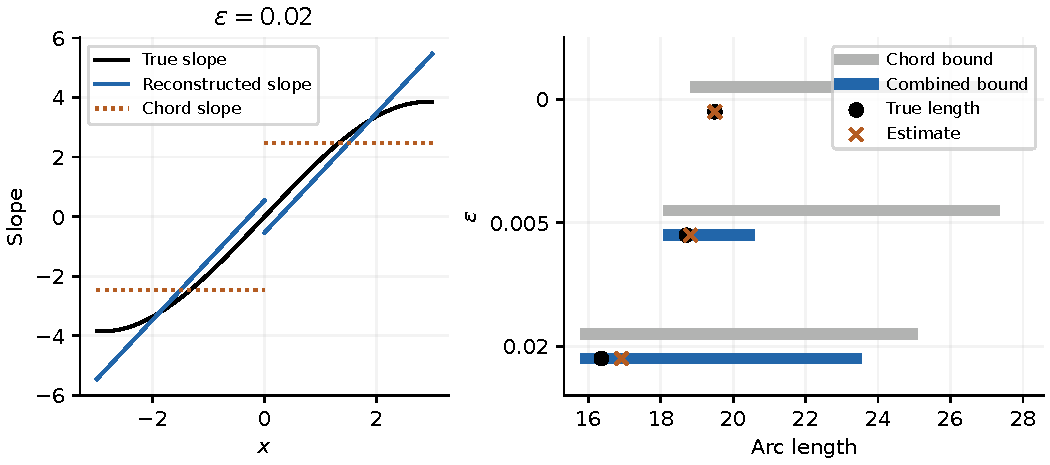
\includegraphics[width=.97\linewidth]{figures/angle_certificate.pdf}
\par\smallskip
\begin{minipage}{.95\linewidth}\small
\textbf{Figure 2.} Left, true, chord, and reconstructed slopes at
$\varepsilon=0.02$. Right, chord and combined bounds. Circles mark true
lengths and crosses mark $\widehat L$. Three samples suffice in each case.
\end{minipage}
\end{minipage}\par\medskip

\notesubsection{Interpretation and scope}
The independent bound $M$ restricts unresolved bending between vertices.
Here $M$ bounds the derivative of graph slope. Euclidean curvature is
$|f''|/(1+f'^2)^{3/2}$, so a curvature bound would need additional slope
information to supply this assumption.
A smooth bump can otherwise increase length while preserving every chord
angle. Setting $M=|m_2-m_1|/h$ from the samples gives only a necessary
lower bound and cannot justify exact recovery. Higher-order length
estimation has an established literature \cite{floater}. The contribution
developed here is inequality \eqref{eq:main}, with historical priority open.


\begingroup\footnotesize
\begin{thebibliography}{3}
\footnotesize
\setlength{\itemsep}{0pt}
\bibitem{landers} J. R. Landers, \emph{Consequences of Minimum Distance
in Mathematics and Physics} (2026), sections on the distance gap and
surviving triangles. Repository manuscript.
\bibitem{triangles} J. R. Landers, \emph{How large must a triangle be
to survive? Minimum-distance exclusion under two sampling laws} (2026).
Repository companion note; context on shortest-side constraints.
\bibitem{floater} M. S. Floater, A. F. Rasmussen, and U. Reif,
\emph{Extrapolation methods for approximating arc length and surface area},
Numerical Algorithms (2007). \href{https://doi.org/10.1007/s11075-007-9095-1}{doi:10.1007/s11075-007-9095-1}.
\end{thebibliography}
\endgroup
\end{document}
